\documentclass[11pt, aspectratio=169]{beamer}
\usetheme{Madrid}
\usefonttheme{serif}

\usepackage[utf8]{inputenc}
\usepackage[T1]{fontenc}
\usepackage{subcaption}
\usepackage{cite}
\usepackage{amsmath}
\usepackage{amsfonts}
\usepackage{amssymb}
\usepackage{graphicx}
\usepackage{csquotes}

\usepackage[english]{babel}

\DeclareMathOperator{\sen}{sen}
\DeclareMathOperator{\tg}{tg}

\setbeamertemplate{caption}[numbered]
\usepackage[font=small,labelfont=bf]{caption}
\author[Group MNIST]{Group MNIST}
\title{Seminar: Image Segmentation Based on Visual Prompt}
% Informe o seu email de contato no comando a seguir
% Por exemplo, alcebiades.col@ufes.br
\newcommand{\email}{email}
%\setbeamercovered{transparent} 
\setbeamertemplate{navigation symbols}{} 
\logo{
\includegraphics[scale=0.06]{imagens/hcmus_logo.png}} 
\institute[]{VNUHCM - University of Science} 
\date{\today} 
%\subject{}

% ---------------------------------------------------------
% Selecione um estilo de referência
\bibliographystyle{apalike}

%\bibliographystyle{abbrv}
%\setbeamertemplate{bibliography item}{\insertbiblabel}
% ---------------------------------------------------------

% ---------------------------------------------------------
% Incluir os slides nos quais as referências foram citadas
%\usepackage[brazilian,hyperpageref]{backref}

%\renewcommand{\backrefpagesname}{Citado na(s) página(s):~}
%\renewcommand{\backref}{}
%\renewcommand*{\backrefalt}[4]{
%	\ifcase #1 %
%		Nenhuma citação no texto.%
%	\or
%		Citado na página #2.%
%	\else
%		Citado #1 vezes nas páginas #2.%
%	\fi}%
% ---------------------------------------------------------

\begin{document}

\begin{frame}
\titlepage
\end{frame}

\section*{Members}
\begin{frame}{Members}
    \begin{center}
      \begin{tabular}{@{}l@{}}
          23122008 - Mai Duc Minh Huy\\
          23122024 - Chung Tin Dat
        \end{tabular}
    \end{center}
\end{frame}

\begin{frame}{Table of contents}
\tableofcontents
\end{frame}

\section{Introduction}
\subsection{General Background}
\begin{frame}{General Background}
	\begin{columns}
		\begin{column}{0.6\linewidth}
			Image segmentation is a fundamental task in computer vision that involves partitioning a digital image into multiple	segments or sets of pixels, often corresponding to different objects or parts of objects.\\
			The goal is to simplify or change the representation of an image into something that is more meaningful and easier to analyze.
		\end{column}
		
		\begin{column}{0.35\linewidth}
			\begin{figure}
				\centering
				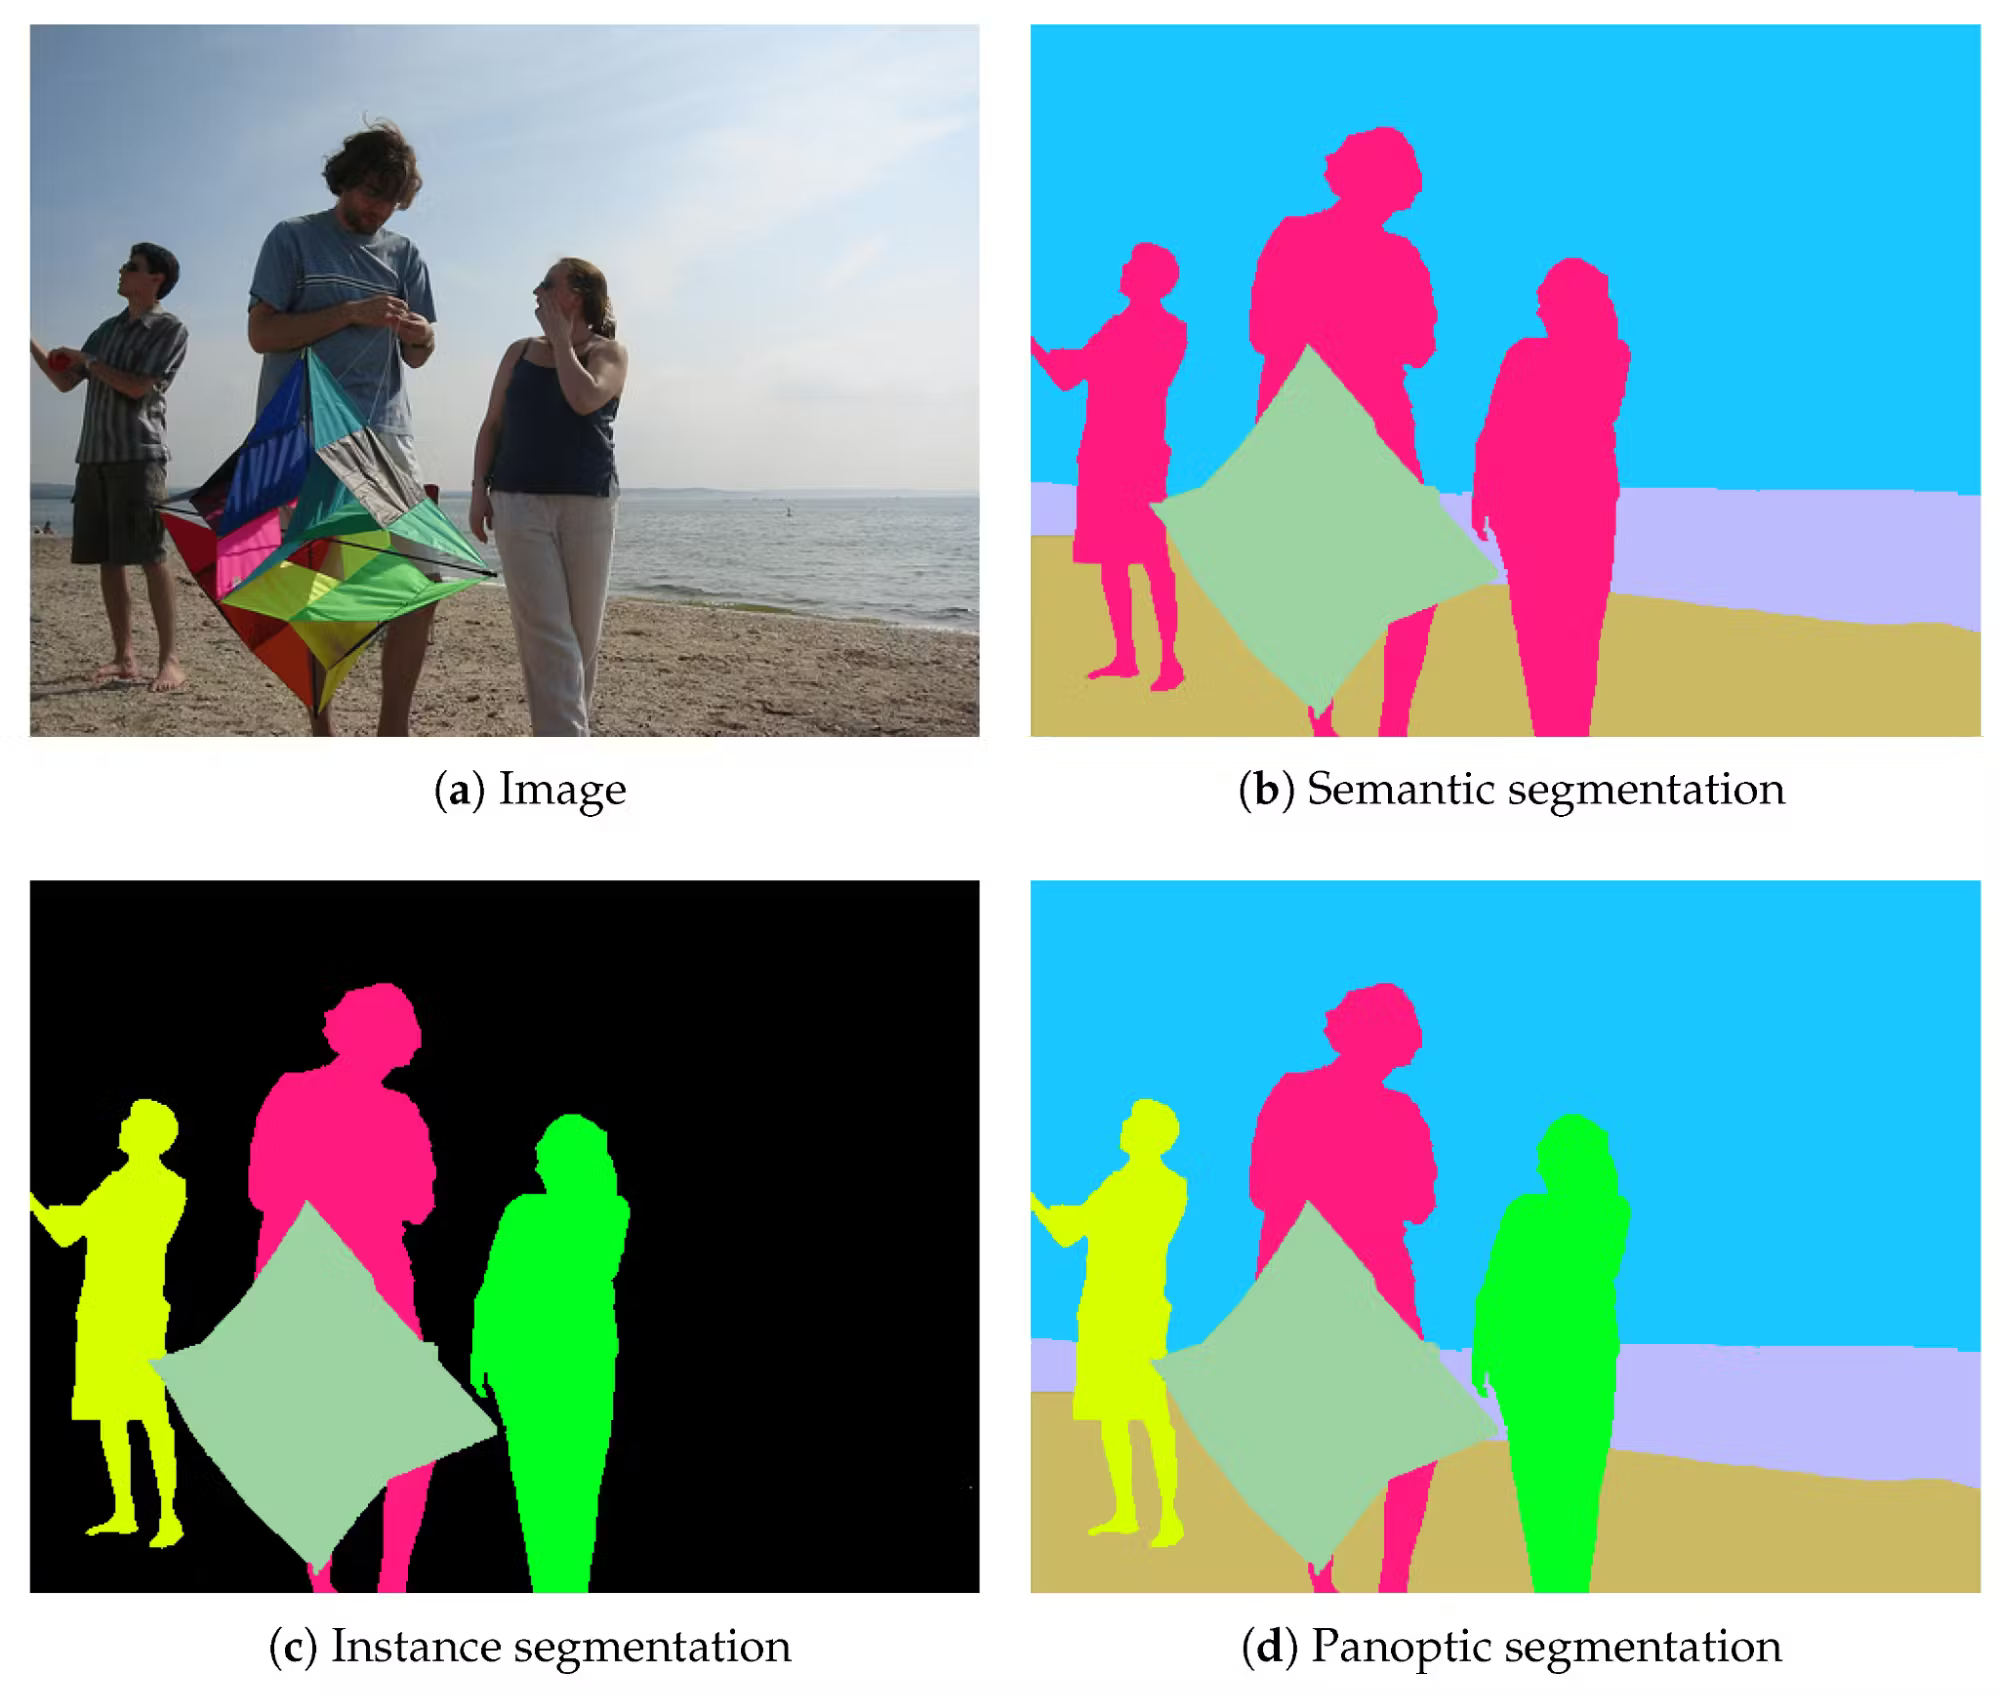
\includegraphics[width=1\linewidth]{imagens/segmentation_example.png}
			\end{figure}
		\end{column}
	\end{columns}
\end{frame}

\begin{frame}{General Background}
	Visual prompts are user-provided graphical inputs—such as clicks, boxes, or lines that "tell" a computer vision algorithm where to focus or what specific object to process.
	\begin{itemize}
		\item \textbf{Points (Clicks): }The user clicks on a specific object (positive click) or background (negative click).
		\item \textbf{Bounding Boxes: }The user drags a rectangle around the object. This gives the algorithm a clear size and location limit.
		\item \textbf{Scribbles/Strokes: }The user draws a rough line over the object.
	\end{itemize}
	\begin{center}
		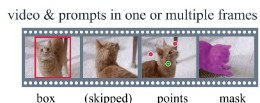
\includegraphics[width=0.6\linewidth]{imagens/Promptable-Visual-Segmentation.jpg}
	\end{center}
\end{frame}

\begin{frame}{General Background}
	The history of this field can be broadly divided into two distinct eras.
	\begin{itemize}
		\item \textbf{The Pre-Deep Learning Era: Seed-Based and Energy Models}
		
		\item \textbf{The Deep Learning Era: From Weak Supervision to Interaction}
	\end{itemize}
\end{frame}

\begin{frame}{The Pre-Deep Learning Era: Seed-Based and Energy Models}
	Before the rise of neural networks, interactive segmentation relied on mathematical frameworks where user inputs acted as "seeds" or constraints for optimization algorithms. These methods focused on low-level features like color gradients and pixel connectivity: \pause \\
	Prominent methods from
	this period include:
	\begin{itemize}
		\item Watershed
		\item Active Contour
		\item Grab Cut
		\item Region Growing
		
	\end{itemize} \pause
	The prompt does not provide "understanding" of the object; it simply tells the math where to start calculating and what color values to look for nearby.
\end{frame}

\begin{frame}{The Deep Learning Era: From Weak Supervision to Interaction}
	The integration of Convolutional Neural Networks (CNNs) allowed models to learn semantic context, making visual prompts significantly more powerful and robust to noise.\pause \\
	Key milestones include:
	\begin{itemize}
		\item Box Sup
		\item Scribble Sup
		\item Deep Extreme Cut
		\item Segment Anything
	\end{itemize}
\end{frame}

\subsection{Motivation}
\begin{frame}{Motivation}
	The drive to advance image segmentation stems from both scientific inquiry and practical necessity. \\
	Scientifically,
	\begin{itemize}
		\item Segmentation addresses a fundamental question in perception: while image classification tells us what is in an image, segmentation answers where it is, down to the pixel level; segmentation helps reveal how an image is organized by separating it into meaningful regions.
		
		\item Many methods in computer vision rely on segmented regions as inputs. Examples include object detection, recognition, tracking, 3D reconstruction, and medical image analysis. Better segmentation improves the performance of these tasks.
	\end{itemize}
\end{frame}

\begin{frame}{Motivation}
	Practically, segmentation is an enabling technology for a multitude of real-world applications.
\end{frame}

\begin{frame}{Motivation}
	
	\begin{columns}[T]
		
		% --- LEFT COLUMN ---
		\begin{column}{0.5\textwidth}
			
			% TOP-LEFT CELL
			\textbf{Autonomous Driving}\par
			\begin{center}
				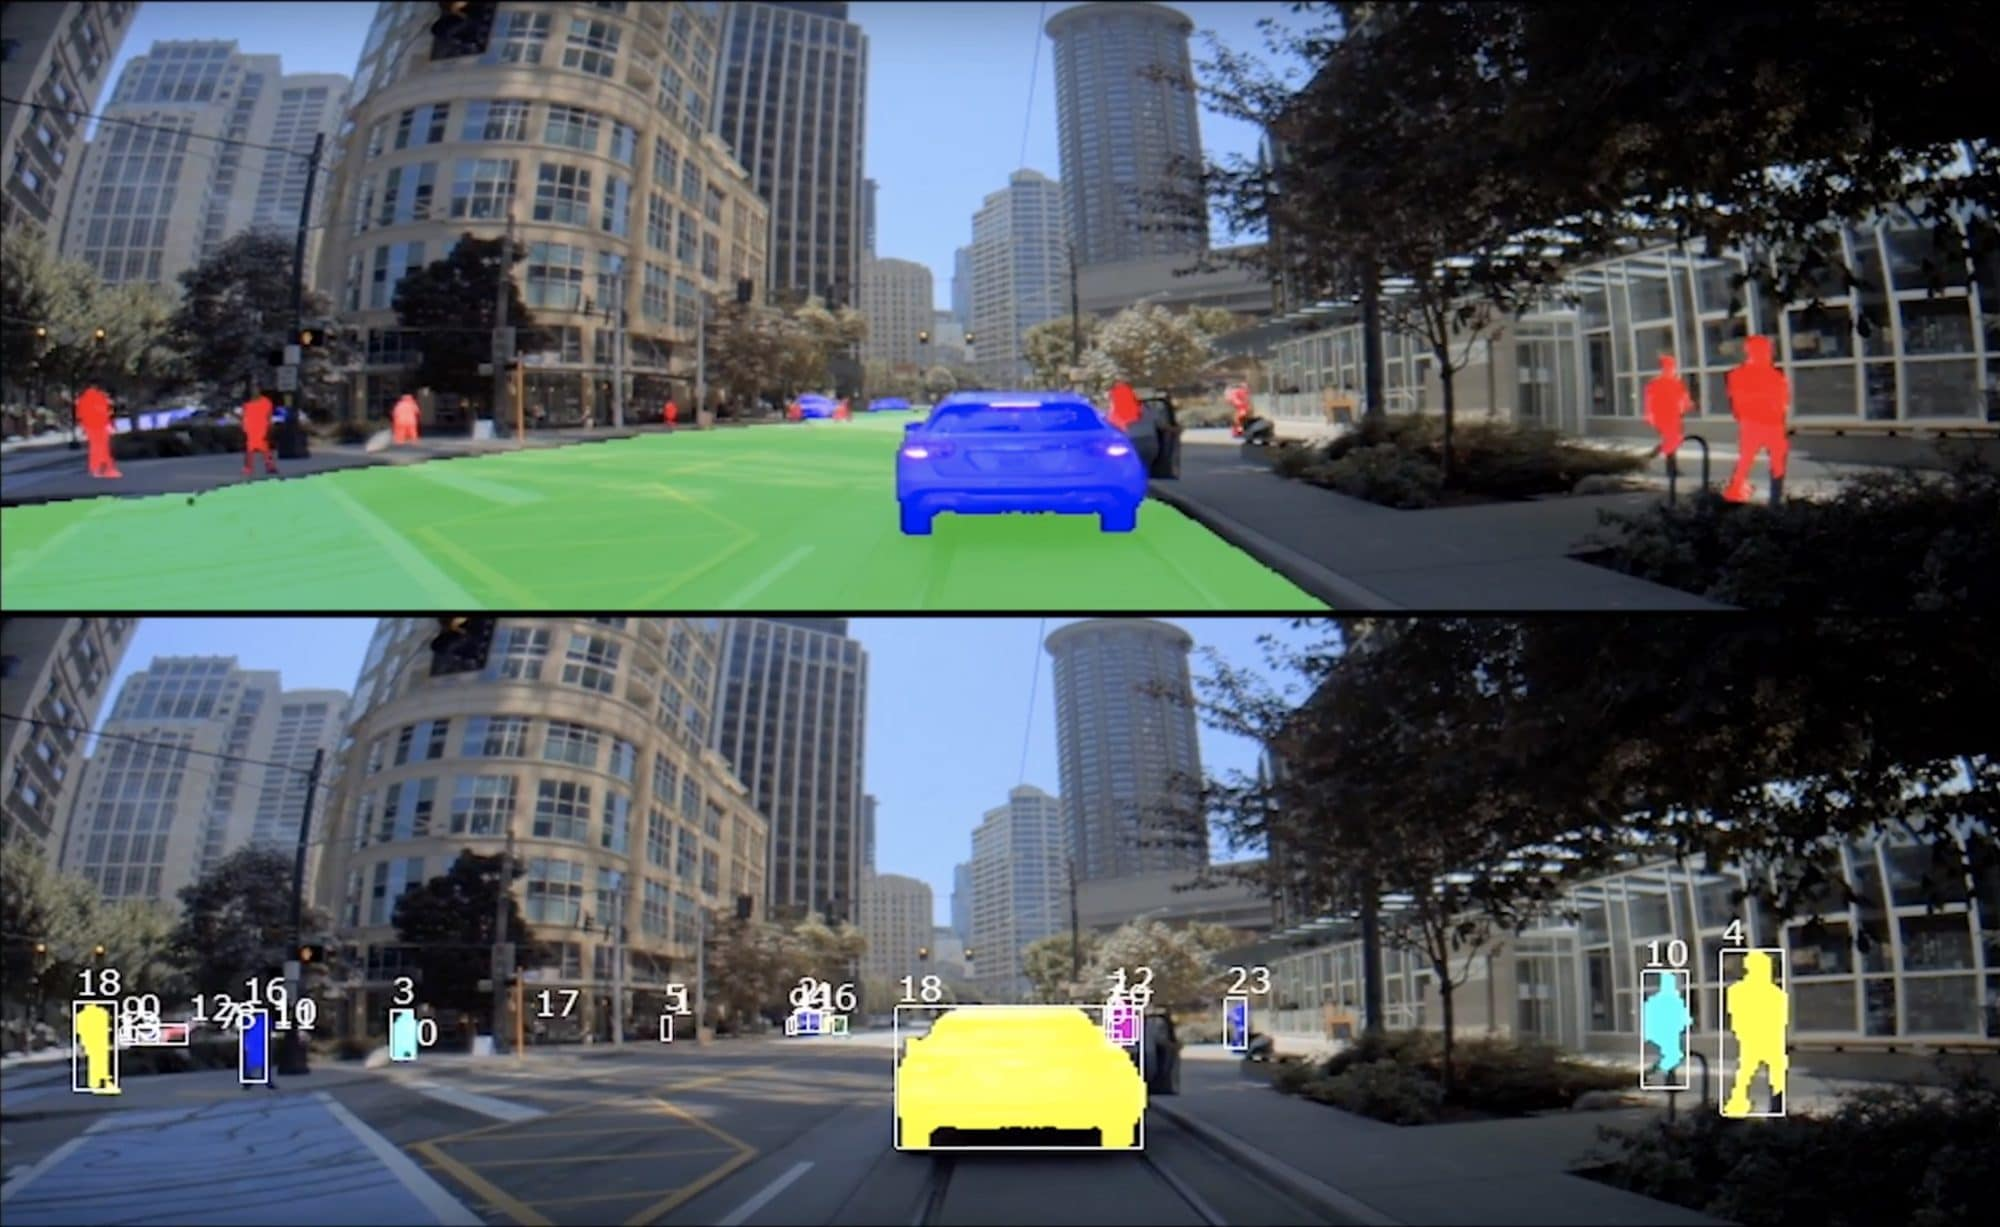
\includegraphics[height=0.25\textheight]{imagens/autonomous.jpg}
				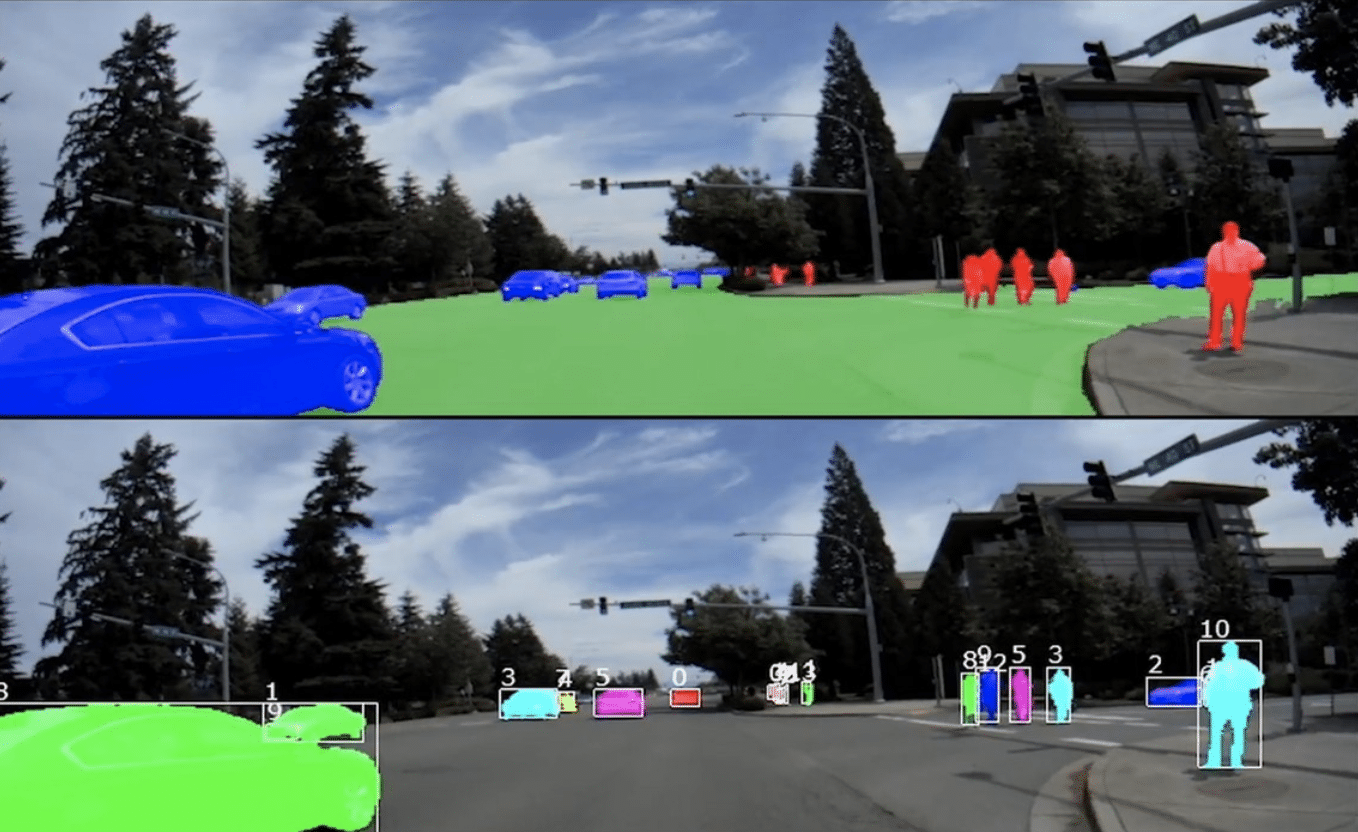
\includegraphics[height=0.25\textheight]{imagens/autonomous_2.jpg}
			\end{center}
			
			\vfill % Adds space between the top and bottom cells
			
			% BOTTOM-LEFT CELL
			\textbf{Surveillance}\par
			\begin{center}
				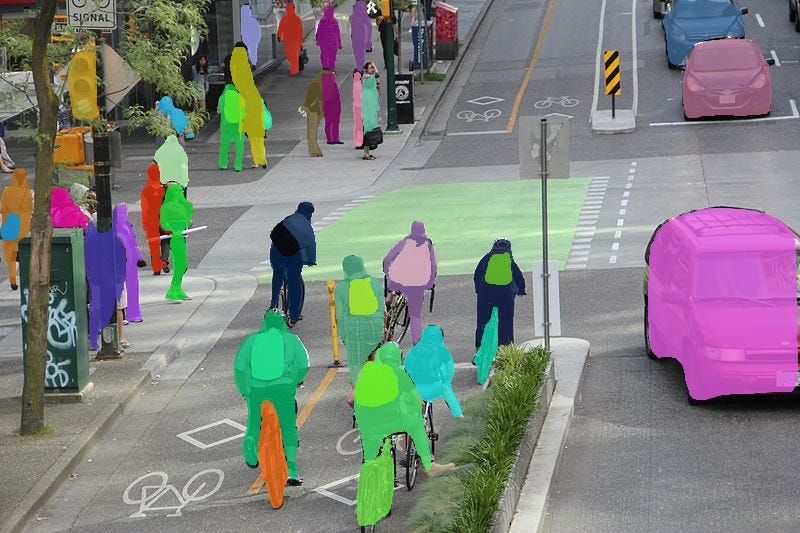
\includegraphics[height=0.25\textheight]{imagens/surveillance.jpg}
				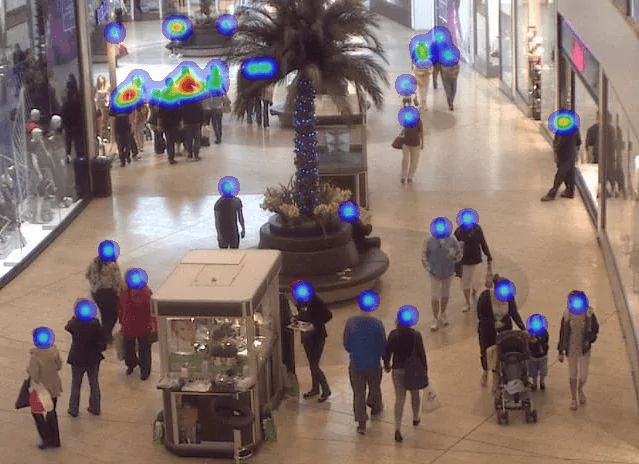
\includegraphics[height=0.25\textheight]{imagens/surveillance_2.png}
			\end{center}
			
		\end{column}
		
		% --- RIGHT COLUMN ---
		\begin{column}{0.5\textwidth}
			
			% TOP-RIGHT CELL
			\textbf{Medical Imaging}\par
			\begin{center}
				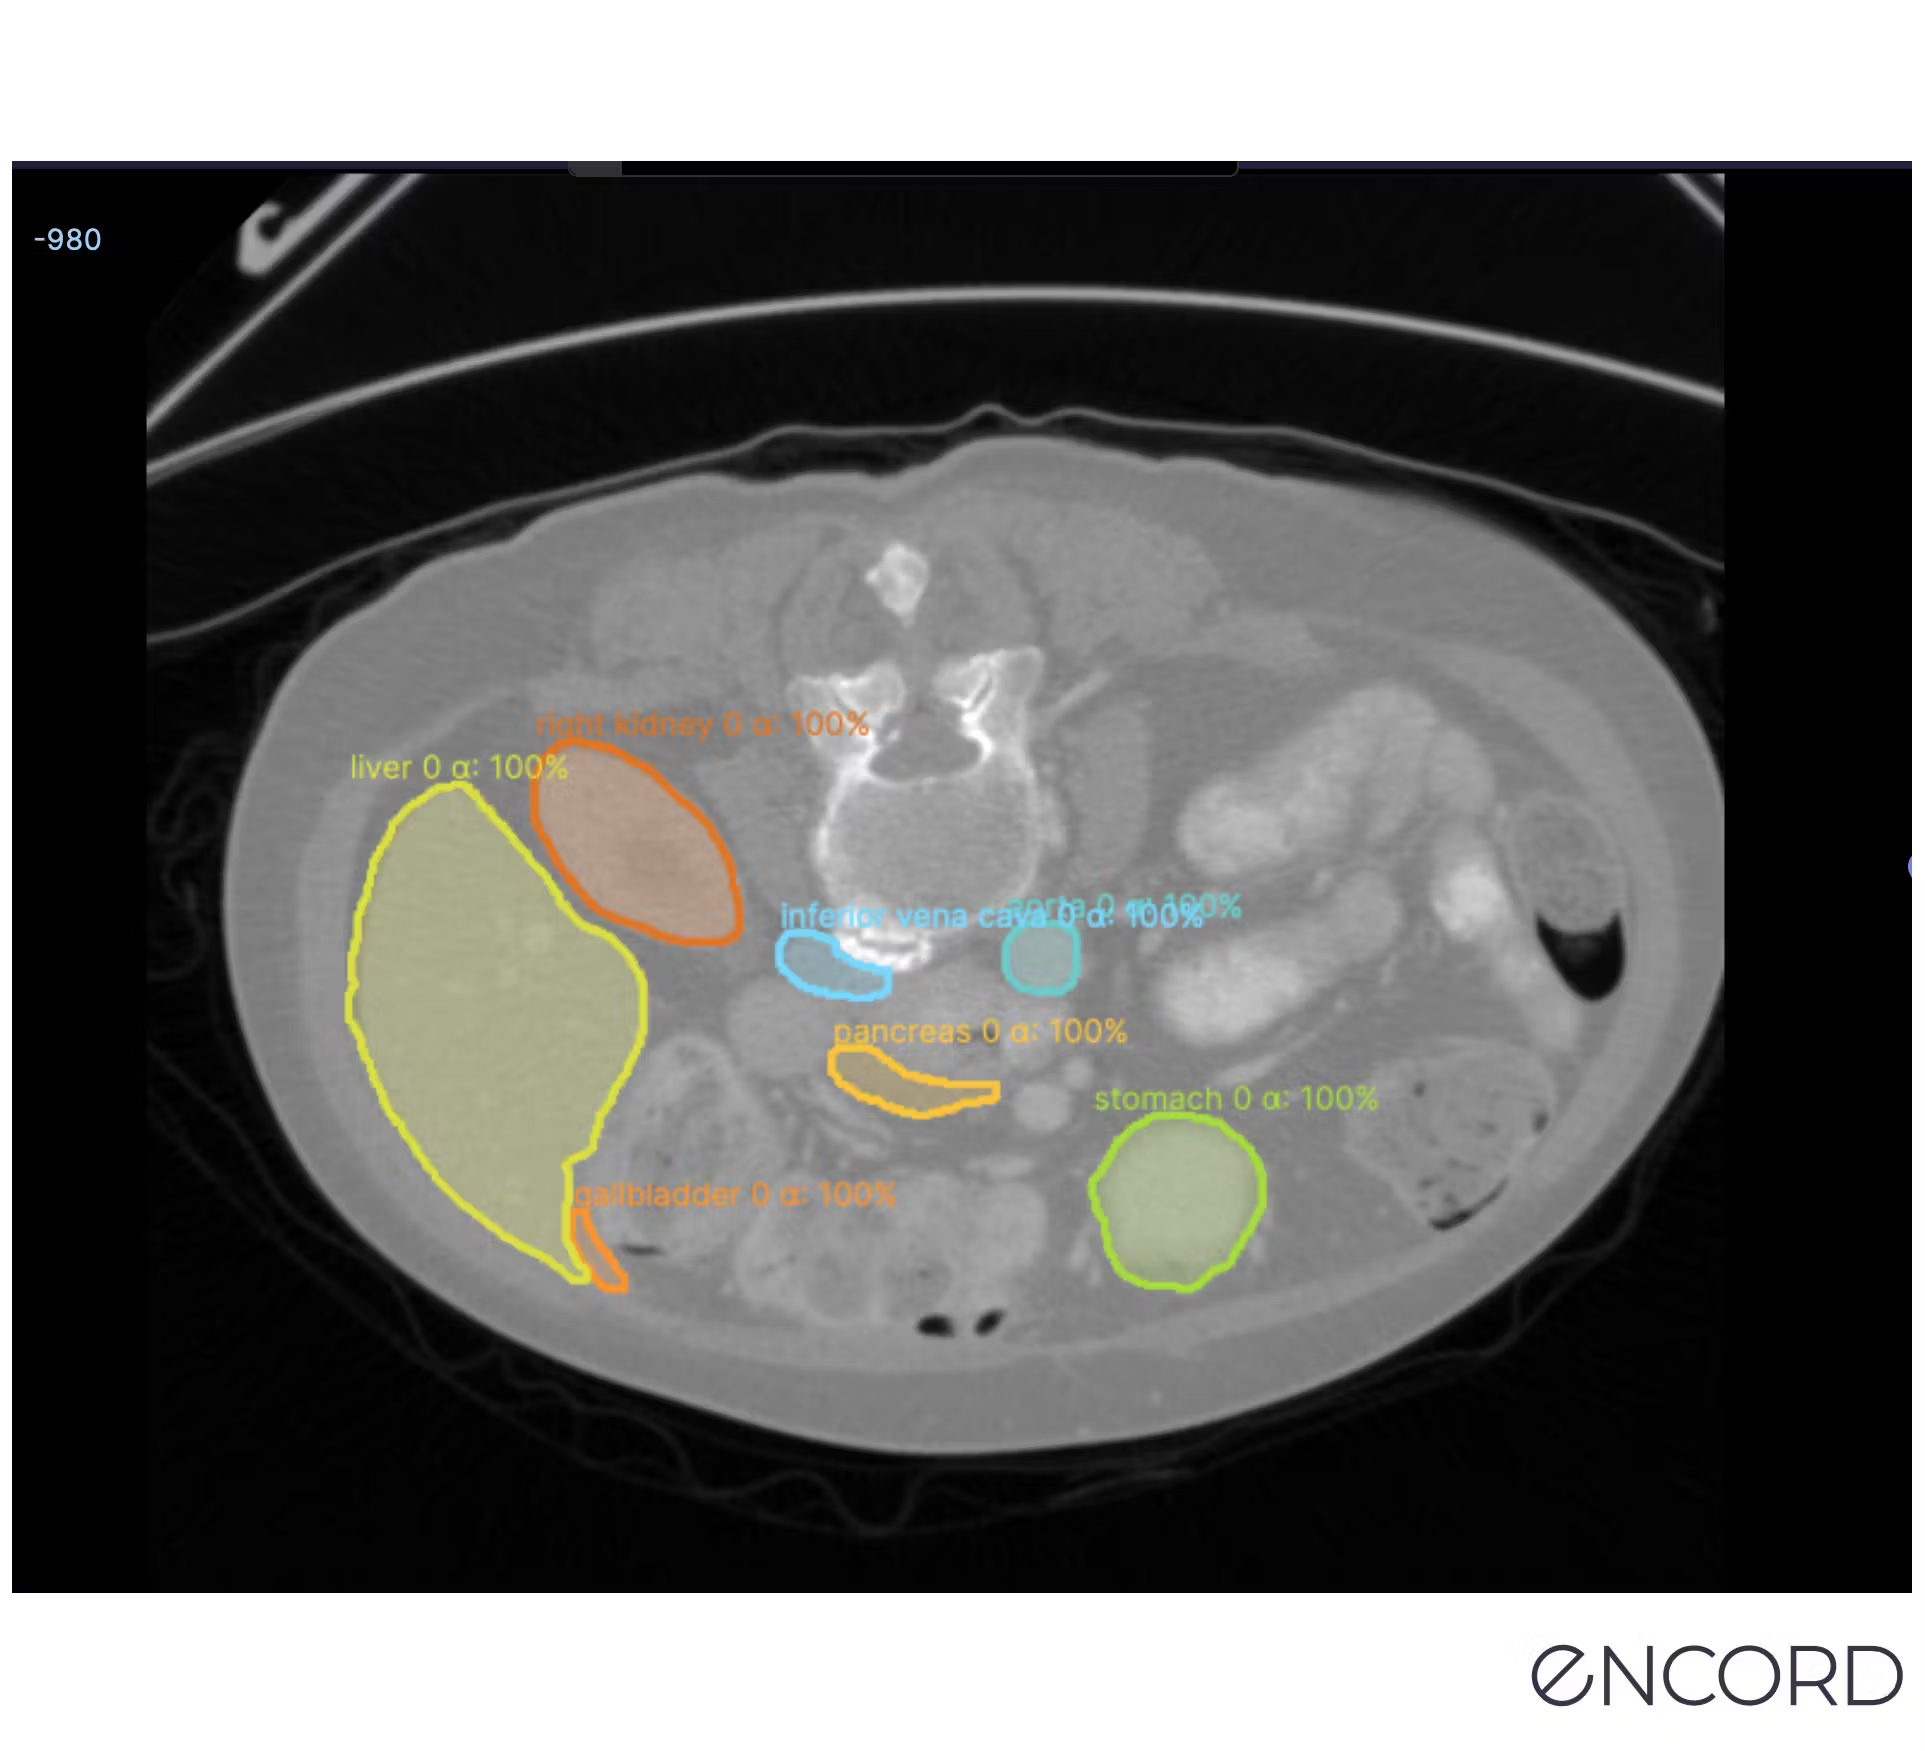
\includegraphics[height=0.25\textheight]{imagens/medical.png}
				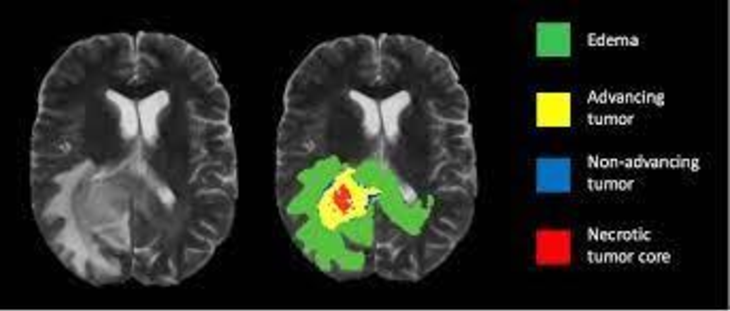
\includegraphics[height=0.25\textheight]{imagens/medical_2.png}
			\end{center}
			
			\vfill % Adds space between the top and bottom cells
			
			% BOTTOM-RIGHT CELL
			\textbf{Object Tracking}\par
			\begin{center}
				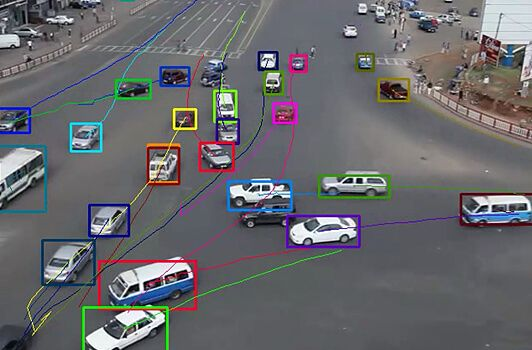
\includegraphics[height=0.25\textheight]{imagens/detection_tracking.jpeg}
				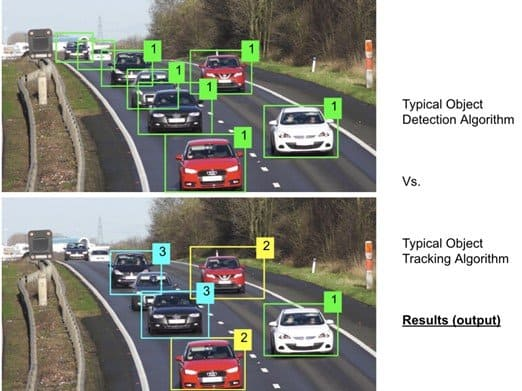
\includegraphics[height=0.25\textheight]{imagens/tracking.jpg}
			\end{center}
			
		\end{column}
		
	\end{columns}
\end{frame}


\begin{frame}{Motivation}
	\textbf{Digital Photograph}\\
	\begin{center}
		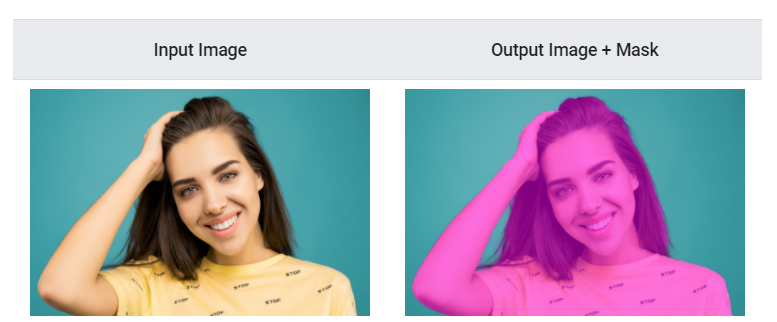
\includegraphics[width=0.5\linewidth]{imagens/photograph_1.png}
		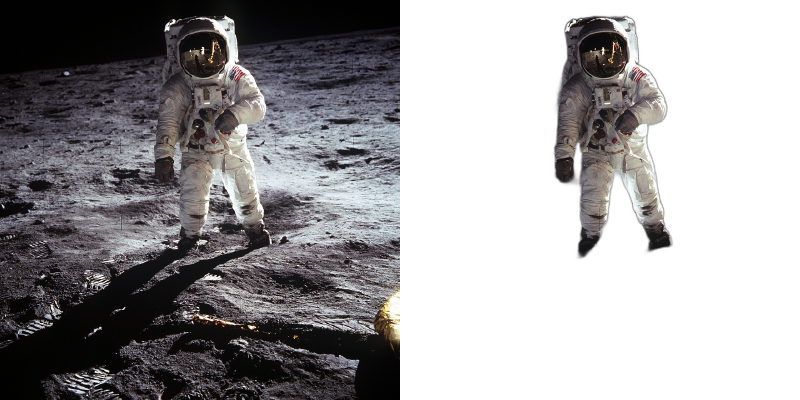
\includegraphics[width=0.4\linewidth]{imagens/photograph_2.png}
	\end{center}
\end{frame}

\begin{frame}{Motivation}
	
	\textbf{Industrial Inspection}\\
	\begin{center}
		\begin{columns}
			\begin{column}{0.3\linewidth}
				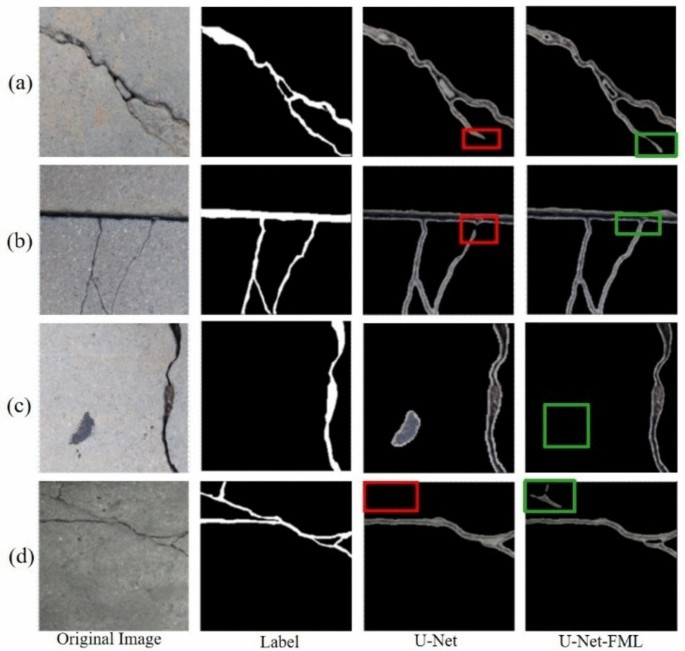
\includegraphics[width=\linewidth]{imagens/industrial_1.jpg}
			\end{column}
			
			\begin{column}{0.7\linewidth}
				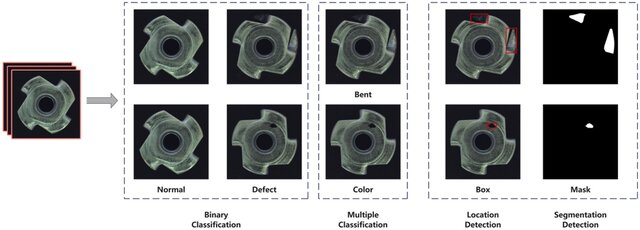
\includegraphics[width=\linewidth]{imagens/industrial_2.jpg}
			\end{column}
		\end{columns}
	\end{center}
		
\end{frame}

\begin{frame}{Motivation}
	\textbf{Segment Anything Model (SAM)}
	\begin{displayquote}
		“In this work, our goal is to build a foundation model
		for image segmentation.”
	\end{displayquote}
	
\end{frame}

\subsection{Problem Statement}
\begin{frame}{Problem Statement}
	Image segmentation is the task of grouping pixels that belong to a common semantic object and separating them from other objects and the background. \\
	The core principle of segmentation is guided by two criteria: pixels within the same group should be as similar as possible, while pixels belonging to different groups should be as distinct as possible. \\
	In essence, the task simulates the human cognitive ability to transform raw, unstructured visual data into a structured representation of distinct entities.
\end{frame}

\begin{frame}{Problem Statement}
	Let $\Omega \subset R ^2$ be the image domain and $I: \Omega \rightarrow R ^k$ the image.\\
	A segmentation is a partition\\
	\begin{center}
		$\Omega = \cup _{i=1}^K \Omega _i \qquad \Omega _i \cap \Omega _j = \emptyset$ for $i \ne j$
	\end{center}
	such that pixels within each region share similar properties according to some criterion.
\end{frame}

\begin{frame}{Problem Statement}
	For a modern promptable segmentation system, the problem can be formally defined by its inputs and outputs.
	
	\begin{columns}[T]
		\begin{column}{0.5\textwidth}
			\begin{itemize}
				\item \textbf{Input:}  An image and a ”visual prompt” that specifies the object of interest. This prompt can take various forms, such as a point (or multiple points) on the object, a bounding box enclosing it, or even a rough mask.
				\item \textbf{Output:} One or more segmentation masks for the object(s) indicated by the prompt, along with a confidence
				score for each mask. 
			\end{itemize}
		\end{column}
		
		\begin{column}{0.5\textwidth}
			\begin{figure}
				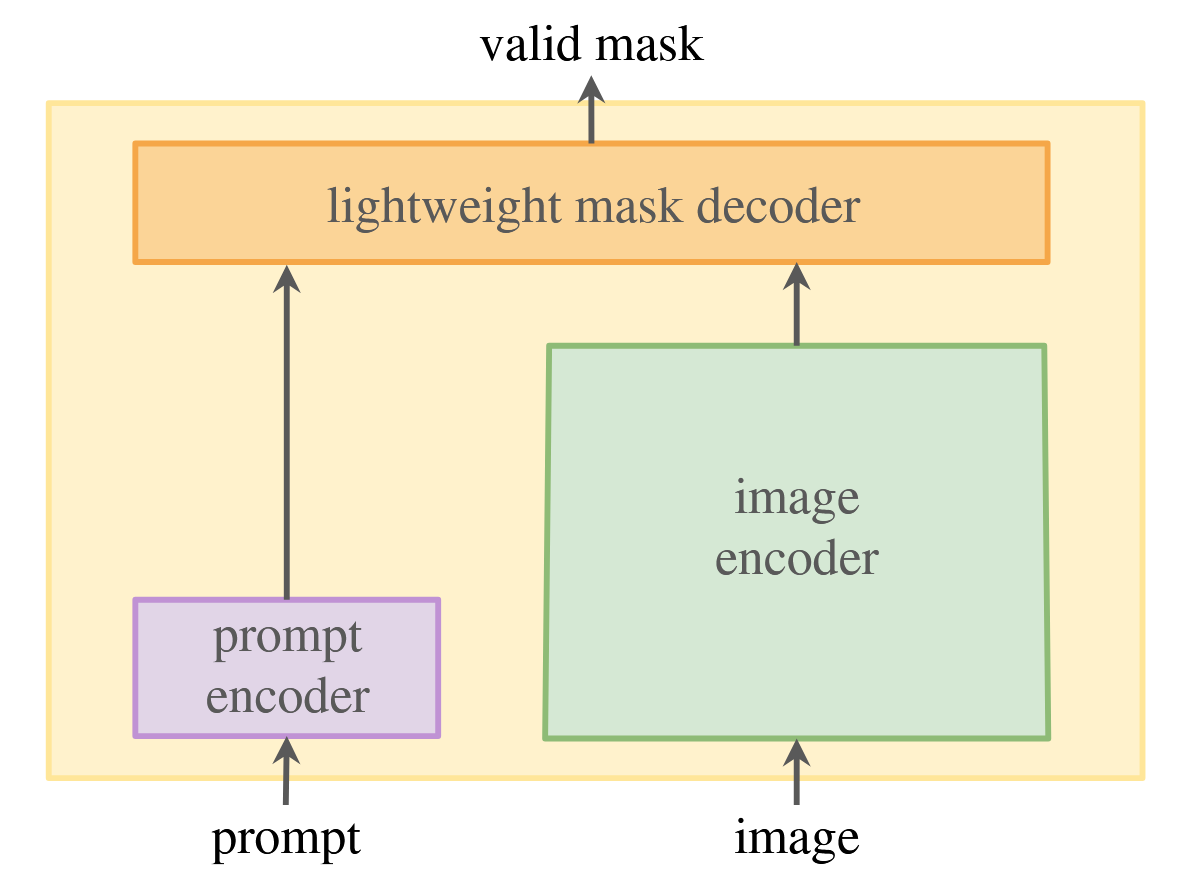
\includegraphics[width=0.8\textwidth]{imagens/framework.png}
			\end{figure}

		\end{column}
	\end{columns}
\end{frame}

\section{Related Works}

\subsection{Traditional Methods}

\begin{frame}{Traditional Methods} % Mechanics
	\begin{table}[h]
		\centering
		\begin{tabular}{|l|p{10cm}|}
			\hline
			\textbf{Methods} & \textbf{Mechanics} \\ \hline
			Watershed & Flooding process on gradient topography with controlled basins. \\ \hline
			Active Contour & Energy minimizing curve driven by internal smoothness and image forces. \\ \hline
			Grab Cut & Local similarity expansion based on pixel intensity or color distance. \\ \hline
			Region Growing & Probabilistic graph cut with iterative foreground background modeling. \\ \hline
		\end{tabular}
	\end{table}
\end{frame}

\begin{frame}{Traditional Methods} % Methodology
	\begin{table}[h]
		\centering
		\begin{tabular}{|l|p{10cm}|}
			\hline
			\multirow{}{\textbf{Methods}} & \textbf{Methodology} \\ \cline{2-2} 
			& \textbf{Stage 1: Input preparation} \\ \hline
			
			Watershed 
			& Image gradient, foreground and background markers. \\ \hline
			
			Active Contour
			& Image as continuous energy field, initial contour. \\ \hline
			
			Grab Cut
			& Image as graph with color distributions (GMMs), bounding box. \\ \hline
			
			Region Growing
			& Image as pixel grid with feature vectors, seed pixels. \\ \hline
			
		\end{tabular}
	\end{table}
\end{frame}

\begin{frame}{Traditional Methods} % Methodology
	\begin{table}[h]
		\centering
		\begin{tabular}{|l|p{5cm}|p{5cm}|}
			\hline
			\textbf{Methods} & \multicolumn{2}{c|}{\textbf{Methodology}} \\ \cline{2-3}
			& \textbf{Stage 2: Propagation/Optimization} & \textbf{Stage 3: Final labeling} \\ \hline
			
			Watershed 
			& Flooding until basins meet.
			& Watershed lines form region boundaries. \\ \hline
			
			Active Contour
			& Iterative energy minimization via curve evolution.
			& Final curve represents object boundary. \\ \hline
			
			Grab Cut
			& Repeated min cut optimization with model updates.
			& Cut defines segmentation boundary. \\ \hline
			
			Region Growing
			& Iterative neighbor expansion.
			& Region boundary from grown region. \\ \hline
			
		\end{tabular}
	\end{table}
	
\end{frame}

\begin{frame}{Traditional Methods} % Contribution
	\begin{table}[h]
		\centering
		\begin{tabular}{|l|p{10cm}|}
			\hline
			\textbf{Methods} & \textbf{Contribution} \\ \hline
			
			Watershed & Introduced topographic interpretation of images and marker controlled segmentation to reduce over segmentation. \\ \hline
			
			Active Contour & Formalized segmentation as energy minimization over curves and influenced decades of variational methods. \\ \hline
			
			Grab Cut & Demonstrated practical interactive segmentation with probabilistic modeling. \\ \hline
			
			Region Growing & Established seed based interactive segmentation. \\ \hline
			
		\end{tabular}
	\end{table}
\end{frame}

\begin{frame}{Traditional Methods} % Limitation
	\begin{table}[h]
		\centering
		\begin{tabular}{|l|p{10cm}|}
			\hline
			\textbf{Methods} & \textbf{Limitations} \\ \hline
			Watershed & Sensitive to noise and gradient quality. \\ \hline
			
			Active Contour & Struggles with concave boundaries and weak edges. \\ \hline
			
			Grab Cut & Assumes color separability between foreground and background; fails when distributions overlap. \\ \hline
			
			Region Growing & Highly sensitive to noise and intensity variation, leakage occurs at weak boundaries. \\ \hline
			
		\end{tabular}
	\end{table}
\end{frame}

\subsection{Deep Learning Methods}

\begin{frame}{Deep Learning Methods} % Mechanics
	\begin{table}[h]
		\centering
		\begin{tabular}{|l|p{10cm}|}
			\hline
			\textbf{Technique} & \textbf{Mechanics} \\ \hline
			
			Box Sup
			& Unsupervised methods to generates hundreds of potential mask shapes (candidate segments), bounding box is used to filter these candidates. \\ \hline
			
			Scribble Sup
			& Image is divided into super pixels, use Graph Cuts optimization to label the unmarked pixels. \\ \hline
			
			Deep Extreme Cut
			& Heatmap from extreme points, CNN extracts feature specifically on the areas highlighted by the heatmap. \\ \hline

			Segment Anything
			& Cross attention between image embedding and prompt embedding. \\ \hline			
		\end{tabular}
	\end{table}
\end{frame}

\begin{frame}{Deep Learning Methods} % Methodology
	\begin{table}[h]
		\centering
		\begin{tabular}{|l|p{5.5cm}|p{5.5cm}|}
			\hline
			\textbf{Technique} & \multicolumn{2}{c|}{\textbf{Methodology}} \\ \cline{2-3}
			& \textbf{Image representation} & \textbf{Prompt encoding} \\ \hline
			
			Box Sup
			& CNN feature maps extracted from region proposals and full images.
			& Bounding boxes converted into soft foreground background supervision using objectness and low level segmentation cues. \\ \hline
			
			Scribble Sup
			& CNN feature maps over full image.
			& Scribbles transformed into dense label maps via graph based or CRF propagation. \\ \hline
			
			Deep Extreme Cut
			& CNN encodes image appearance along with spatial context.
			& Extreme points encoded as distance maps concatenated with image channels. \\ \hline
			
			Segment Anything
			& Vision transformer generates dense image embeddings.
			& Prompts encoded into tokens representing points, boxes, or masks. \\ \hline
			
		\end{tabular}
	\end{table}
\end{frame}

\begin{frame}{Deep Learning Methods} % Methodology
	\begin{table}[h]
		\centering
		\begin{tabular}{|l|p{10cm}|}
			\hline
			\multirow{}{\textbf{Methods}} & \textbf{Methodology} \\ \cline{2-2} 
			& \textbf{Mask decoding} \\ \hline
			
			Box Sup
			& CNN trained on pseudo masks predicts dense semantic segmentation masks. \\ \hline
			
			Scribble Sup
			& CNN outputs semantic masks learned from propagated pseudo labels. \\ \hline
			
			Deep Extreme Cut
			& Single pass CNN inference produces object mask. \\ \hline
			
			Segment Anything
			& Transformer based mask decoder predicts multiple candidate masks with confidence scores. \\ \hline
		\end{tabular}
	\end{table}
\end{frame}

\begin{frame}{Deep Learning Methods} % Contribution
	\begin{table}[h]
		\centering
		\begin{tabular}{|l|p{10cm}|}
			\hline
			\textbf{Technique} & \textbf{Contribution} \\ \hline
			
			Box Sup
			& It effectively combined traditional "region proposal" methods (unsupervised) with deep learning (supervised), allowing the network to learn shapes without ever seeing a ground truth mask. \\ \hline
			
			Scribble Sup
			& It successfully integrated a Graphical Model (Graph Cut) into the deep learning pipeline. The graph propagates the scribble information to nearby pixels based on color/texture, creating a dense mask to train the CNN. \\ \hline
			
			Deep Extreme Cut
			& It showed that annotating extreme points is 5x faster than drawing polygons but yields results that are nearly as good as fully supervised learning. \\ \hline
			
			Segment Anything
			& First truly general purpose segmentation foundation model. Enables interactive segmentation, automatic segmentation, and box guided segmentation in one model. \\ \hline
			
		\end{tabular}
	\end{table}
\end{frame}

\begin{frame}{Deep Learning Methods} % Limitation
	\begin{table}[h]
		\centering
		\begin{tabular}{|l|p{11cm}|}
			\hline
			\textbf{Technique} & \textbf{Limitations} \\ \hline
			
			Box Sup
			& The model is limited by the quality of the candidate generation (MCG/Selective Search). If the proposal algorithm fails to generate a mask that fits the object, the CNN cannot learn it. \\ \hline
			
			Scribble Sup
			& The "propagation" step relies on traditional color and texture similarity. If the object has low contrast, the graph cut fails to spread the label correctly. \\ \hline
			
			Deep Extreme Cut
			& The user must provide exactly 4 points, and they must be the extreme edges. It struggles with objects that have disjoint parts because the extreme points might not capture the empty space in between efficiently. \\ \hline
			
			Segment Anything
			& High computational cost during preprocessing due to large encoder. Not ideal for pixel perfect tasks such as thin structures or high precision medical boundaries without fine tuning. Mask quality depends on prompt placement. \\ \hline
			
		\end{tabular}
	\end{table}
	
\end{frame}

\section{Methodology}
\subsection{Data Collection}
\begin{frame}{Dataset SA-1B}
	The fundamental challenge in building a foundation model for segmentation is the lack of web-scale segmentation data.\\
	Segmentation masks are not naturally occurring and must be manually created.\\
	Traditional approaches would require paying annotators to label billions of masks-economically infeasible and temporally prohibitive.
\end{frame}

\begin{frame}{Dataset SA-1B}
	\textbf{SAM Data Engine:}
	\begin{enumerate}
		\item Assisted Manual Annotation (4.3M Masks from 120K Images)
		\item Semi-Automatic Annotation (5.9M Additional Masks, 180K Images)
		\item Fully Automatic Annotation (1.1B Masks, 11M Images)
	\end{enumerate}
\end{frame}

\begin{frame}{Dataset SA-1B}
	\textbf{1. Assisted Manual Annotation (4.3M Masks from 120K Images):} \\
	Workflow:
	\begin{enumerate}
		\item Professional annotators view an image in a web-based interface.
		\item They click foreground/background points to indicate an object of interest.
		\item SAM's pre-computed image embedding (from MAE-ViT-H) is queried with these prompts.
		\item The lightweight Prompt Encoder and Mask Decoder run in real-time ($< 50$ms), generating an initial mask prediction.
		\item Annotators refine the mask using pixel-precise brush and eraser tools.
		\item The final mask is saved.
	\end{enumerate}
\end{frame}

\begin{frame}{Dataset SA-1B}
	\textbf{Quantitative Dynamics:} \\
	\begin{itemize}
		\item \textbf{Initial annotation time:} 34 seconds per mask (comparable to COCO annotation standards).
		\item \textbf{Model capacity progression:} ViT-B $\rightarrow$ ViT-H during this stage (1 retraining cycle per major improvement).
		\item \textbf{Average masks per image:} $20 \rightarrow 44$ (increased diversity as model improved).
		\item \textbf{Total masks collected:} 4.3M from 120K images.
		\item \textbf{Retraining cycles:} 6 full model retraining iterations.
		\item \textbf{Total masks collected:} 4.3M from 120K images.
	\end{itemize}
\end{frame}

\begin{frame}{Dataset SA-1B}
	\textbf{Efficiency Gain Analysis:} \\
	The $34 \rightarrow 14$ second progression represents a \textbf{6.5$\times$ speedup over COCO standards} (34 seconds here vs. 14 seconds for bounding boxes). This exponential improvement in annotation velocity is crucial for economic feasibility at billion-scale.
\end{frame}

\begin{frame}{Dataset SA-1B}
	\textbf{2. Semi-Automatic Annotation (5.9M Additional Masks, 180K Images):} \\
	Workflow:
	\begin{enumerate}
		\item Train a generic object detector on all masks from Stage 1. This detector outputs bounding boxes regardless of semantic class (object-agnostic proposal generation).
		\item SAM automatically segments high-confidence regions identified by this detector, generating candidate masks.
		\item Annotators are presented with images pre-filled with these automatic masks.
		\item Annotators' task: Label only the \textit{unannotated} objects (those not covered by the automatic masks).
		\item This forces annotators to focus on smaller, more occluded, or semantically ambiguous objects.
	\end{enumerate}
\end{frame}

\begin{frame}{Dataset SA-1B}
	\textbf{Why This Engineering is Critical:} \\
	The semi-automatic stage is a \textbf{curriculum learning} strategy. By automatically handling easy cases and forcing annotators to label hard cases, the model learns a more balanced representation. This is empirically validated: the model's ability to handle edge cases improved significantly from Stage 1 to Stage 2, as evidenced by the diversity metrics.
\end{frame}

\begin{frame}{Dataset SA-1B}
	\textbf{Efficiency Gain Analysis:} \\
	The $34 \rightarrow 14$ second progression represents a \textbf{6.5$\times$ speedup over COCO standards} (34 seconds here vs. 14 seconds for bounding boxes). This exponential improvement in annotation velocity is crucial for economic feasibility at billion-scale.
\end{frame}

\begin{frame}{Dataset SA-1B}
	\textbf{Why stage 2 is needed?}\\
	By automatically handling easy cases and forcing annotators to label hard cases, the model learns a more balanced representation. This is empirically validated: the model's ability to handle edge cases improved significantly from Stage 1 to Stage 2, as evidenced by the diversity metrics.
\end{frame}

\begin{frame}{Dataset SA-1B}
	\textbf{3. Fully Automatic Annotation (1.1B Masks, 11M Images):} \\
	Systematically prompt the model with a regular spatial grid of points ($32 \times 32$), covering the entire image.
	Workflow:
	\begin{enumerate}
		\item Each point is passed as a prompt to the Prompt Encoder.
		\item For each point, SAM predicts \textbf{three masks simultaneously}.
		\item \textbf{Theoretical maximum:} $1024 \text{ points} \times 3 \text{ masks per point} = 3072 \text{ masks per image}$.
	\end{enumerate}
\end{frame}

\begin{frame}{Dataset SA-1B}
	\textbf{Filtering, Deduplication, Non-Maximum Suppression}\\
	\begin{enumerate}
		\item IoU Scoring and Confidence Thresholding
		\item Stability Filtering
		\item Non-Maximum Suppression (NMS)
	\end{enumerate}
\end{frame}

\begin{frame}{Dataset SA-1B}
	\textbf{IoU Scoring and Confidence Thresholding}\\
	\begin{itemize}
		\item For each of the three masks predicted from a grid point, SAM outputs a \textbf{predicted IoU score} (estimated mask quality).
		\item \textbf{Threshold:} Only masks with \textbf{predicted IoU $>$ 0.88} are retained.
		\item \textbf{Rationale:} High IoU threshold ensures only high-quality masks enter the deduplication pipeline.
		\item \textbf{Expected reduction:} From 3072 theoretical outputs, this threshold alone eliminates $\sim$80\% of predictions (keeping only predictions the model is highly confident about).
	\end{itemize}
\end{frame}

\begin{frame}{Dataset SA-1B}
	\textbf{Stability Filtering}\\
	\begin{itemize}
		\item A mask is \textbf{stable} if small perturbations in the model's confidence threshold (e.g., changing the foreground probability threshold from 0.5 to $0.5 \pm \epsilon$) produce similar masks.
		\item \textbf{Operationally:} Threshold the mask's probability map at both 0.5 and 0.5, and compute the IoU between the two resulting binary masks.
		\item If this "stability IoU" is high ($> 0.95$), the mask is kept; otherwise, it is discarded.
		\item \textbf{Why This Matters:} Masks that are brittle (sensitive to small threshold changes) are often segmentation errors or include spurious boundaries. Stability filtering removes low-confidence predictions and keeps robust ones.
		\item \textbf{Further reduction:} $\sim$50\% of remaining masks fail stability checks.
	\end{itemize}
\end{frame}

\begin{frame}{Dataset SA-1B}
	\textbf{Non-Maximum Suppression}\\
	\begin{enumerate}
		\item Sort masks by predicted IoU score.
		\item Select the highest-scoring mask $m_1$.
		\item Foa all remaining masks $m_i$:
		\begin{itemize}
			\item Compute $\text{IoU}(m_1, m_i) = \frac{|m_1 \cap m_i|}{|m_1 \cup m_i|}$ (Jaccard index).
			\item If $\text{IoU}(m_1, m_i) > \text{thresh}_{\text{IoU}}$ (typically 0.7), discard $m_i$ (it is a near-duplicate).
			\item If $\text{IoU}(m_1, m_i) \leq \text{thresh}_{\text{IoU}}$, retain $m_i$ (it is a distinct object).
		\end{itemize}
		\item Repeat on remaining unprocessed masks.
	\end{enumerate}
\end{frame}

\begin{frame}{Dataset SA-1B}
	\textbf{Scale Reduction Summary:}
	\begin{itemize}
		\item \textbf{Start:} 3072 theoretical masks ($32 \times 32$ grid $\times$ 3 outputs per grid cell).
		\item \textbf{After IoU filtering ($>0.88$):} $\sim$600 masks (20\% remain).
		\item \textbf{After stability filtering:} $\sim$300 masks (50\% of IoU-filtered).
		\item \textbf{After NMS ($\text{thresh\_IoU} = 0.7$):} $\mathbf{\sim100 \text{ masks}}$ (final).
	\end{itemize}
	
	\textbf{Final Calculation:}
	\[
	\text{Total SA-1B Masks} = 11\text{M images} \times 100 \text{ masks/image} = 1.1 \text{ B masks}
	\]
\end{frame}

\begin{frame}{Dataset SA-1B}
	\textbf{Why stage 3 is needed?}\\
	A regular grid ensures comprehensive spatial coverage. If an object's boundary passes through or near a grid point, the model will capture it from that point. Objects of varying sizes are covered because the grid is at a fixed, moderate resolution. This is fundamentally different from random point sampling, which can miss objects entirely.
\end{frame}

\begin{frame}{Dataset SA-1B}
	Overall, this three-stage pipeline can be summarized:
	\begin{enumerate}
		\item \textbf{Stage 1} teaches the model to segment \textit{diverse} objects via human guidance.
		\item \textbf{Stage 2} forces the model to learn \textit{challenging} objects via curriculum learning.
		\item \textbf{Stage 3} leverages the improved model to generate \textit{scale} without human cost.
	\end{enumerate}
\end{frame}

\begin{frame}{Segment Anything Model}
	\textbf{Why 3 outputs per prompt?}\\
	Empirical analysis during SAM's development showed that image regions typically have at most three levels of semantic hierarchy (whole $>$ part $>$ sub-part). Predicting three masks covers all common ambiguity scenarios without excessive computation.
\end{frame}

\begin{frame}{Segment Anything Model}
	\textbf{The Output Token Design:}
	\begin{itemize}
		\item The Mask Decoder predicts three masks from a single prompt, ranked by IoU score.
		\item \textbf{Whole object:} The complete, semantically coherent object.
		\item \textbf{Part:} A prominent sub-component (e.g., a wheel on a car, a face on a person).
		\item \textbf{Sub-part:} Fine-grained components (e.g., an eye within a face, a spoke within a wheel).
	\end{itemize}
\end{frame}

\begin{frame}{Segment Anything Model}
	Output token is an embedding vector acts as a query for the final mask prediction (analogous to CLS token in BERT or ViT).\\
	This token gether information about the prompt embeddings and image embeddings to form semantic information required to segment the target object.
\end{frame}

\begin{frame}{Segment Anything Model}
	\begin{center}
		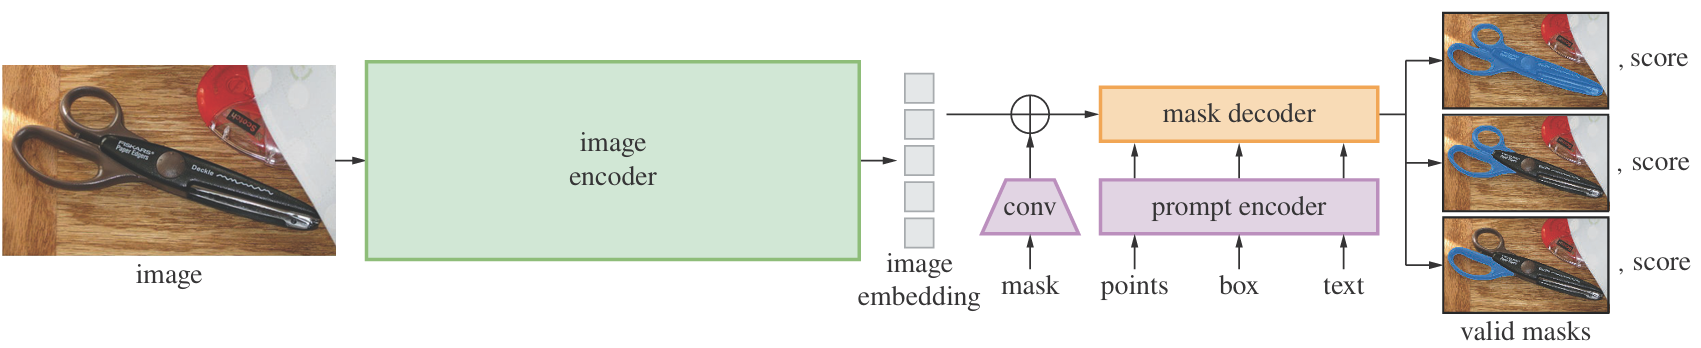
\includegraphics[width=\linewidth]{imagens/sam_architecture.png}
	\end{center}
	\begin{itemize}
		\item Image Encoder: MAE pre-trained Vision Transformer (ViT).
		\item Prompt Encoder: 
		\begin{itemize}
			\item Point, box: Positional encoding summed with learned embeddings for each prompt type.
			\item Mask: Convolution and summed element-wise with the image embedding.
		\end{itemize}
			
	\end{itemize}
\end{frame}

\begin{frame}{Segment Anything Model}
	\begin{itemize}
		\item Mask Decoder:
		\begin{center}
			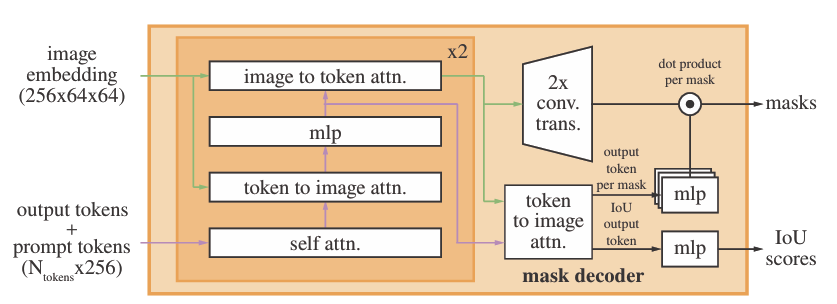
\includegraphics[width=\linewidth]{imagens/mask_decoder.png}
		\end{center}
		
	\end{itemize}
\end{frame}

\begin{frame}{Segment Anything Model}
	\textbf{Key Design:}
	\begin{itemize}
		\item Image Encoder runs \textbf{once per image}, producing a latent embedding.
		\item This embedding is cached.
		\item Prompt Encoder and Mask Decoder run \textbf{every time the user provides a new prompt} on the cached embedding.
		\item Result: 50ms per prompt on CPU in a web browser (no GPU required).
	\end{itemize}
\end{frame}

\begin{frame}{Segment Anything Model}
	In traditional interactive segmentation (e.g., RITM, SimpleClick), the entire network processes the image for each new click, leading to latency. SAM's decoupling means that the first prompt has a cost (cached image encoding) and subsequent prompts are nearly free. For applications with many prompts (e.g., dense instance segmentation with many objects), the amortized cost per object approaches zero.
\end{frame}

\begin{frame}{Segment Anything Model}
	Image Encoder: A Vision Transformer (ViT) processes images by:
	\begin{enumerate}
		\item Dividing the image into non-overlapping patches (typically $16 \times 16$ pixels).
		\item Flattening each patch into a 1D vector and projecting to embedding dimension $d = 768$ (for ViT-B) or $d = 1280$ (for ViT-H).
		\item Adding \textbf{positional embeddings} to inject spatial information.
		\item Processing the sequence of patch embeddings through stacked Transformer layers using self-attention.
	\end{enumerate}
\end{frame}

\begin{frame}{Segment Anything Model}
	Prompt Encoder:
	\textbf{Points (Foreground/Background):}
	
	A point prompt is simply a 2D coordinate $(x, y)$ and a label indicating foreground (+1) or background (-1).
	
	\textbf{Representation:}
	\begin{enumerate}
		\item Convert coordinate to positional encoding (using sinusoidal or learned embeddings).
		\item Embed the foreground/background label using learned embeddings $\mathbf{e}_{\text{fg}}$ and $\mathbf{e}_{\text{bg}}$ (dimension 256).
		\item Sum the positional and semantic embeddings:
		\[ \mathbf{p}_{\text{point}} = PE(x, y) + \mathbf{e}_{\text{label}} \]
	\end{enumerate}
\end{frame}

\begin{frame}{Segment Anything Model}
	Prompt Encoder:
	\textbf{Boxes (Bounding Box Prompts):}
	
	A box is specified by two corners: $(x_{\min}, y_{\min}, x_{\max}, y_{\max})$.
	
	\textbf{Representation:}
	\begin{enumerate}
		\item Generate two "corner points": $(x_{\min}, y_{\min})$ and $(x_{\max}, y_{\max})$.
		\item Encode each corner with distinct learned embeddings ($\mathbf{e}_{\text{top-left}}$, $\mathbf{e}_{\text{bottom-right}}$).
		\item Embed the box as:
		\[ \mathbf{p}_{\text{box}} = [PE(x_{\min}, y_{\min}) + \mathbf{e}_{\text{top-left}}, \quad PE(x_{\max}, y_{\max}) + \mathbf{e}_{\text{bottom-right}}] \]
	\end{enumerate}
\end{frame}

\begin{frame}{Segment Anything Model}
	Prompt Encoder:
	\textbf{Mask (Dense Prompts):}
	
	\textbf{Representation:}
	\begin{enumerate}
		\item Resize the input mask to match the spatial resolution of the Image Embedding (e.g., $256 \times 256$ if image is $1024 \times 1024$).
		\item Apply \textbf{2D convolutions} to extract spatial features:
		\begin{itemize}
			\item Input: Binary mask (single channel).
			\item Conv layers: 3–4 layers with ReLU activations, stride 1.
			\item Output: Feature map of shape $(256 \times 256, C)$ where $C = 256$.
		\end{itemize}
		\item Element-wise sum with the Image Embedding:
		\[ \mathbf{z}_{\text{fused}} = \mathbf{z}_{\text{image}} + \mathbf{z}_{\text{mask}} \]
	\end{enumerate}
\end{frame}

\begin{frame}{Segment Anything Model}
	Mask Decoder: Two-Way Transformer Fusion
	
	\begin{enumerate}
		\item \textbf{Self-attention on prompts:} Prompts attend to themselves to capture relationships between multiple prompts (e.g., if multiple points are provided, they can "communicate").
		\[ \mathbf{A}_{\text{prompt}} = \text{Softmax}\left(\frac{\mathbf{Q}_{\text{prompt}} \mathbf{K}_{\text{prompt}}^T}{\sqrt{d}}\right) \mathbf{V}_{\text{prompt}} \]
		
		\item \textbf{Cross-attention (prompt $\rightarrow$ image):} Prompts query the Image Embedding to extract relevant regions.
		\[ \mathbf{A}_{\text{p2i}} = \text{Softmax}\left(\frac{\mathbf{Q}_{\text{prompt}} \mathbf{K}_{\text{image}}^T}{\sqrt{d}}\right) \mathbf{V}_{\text{image}} \]
	\end{enumerate}
\end{frame}

\begin{frame}{Segment Anything Model}
	Mask Decoder: Two-Way Transformer Fusion
	
	\begin{enumerate}
    	\item \textbf{Cross-attention (image $\rightarrow$ prompt):} Conversely, the Image Embedding queries the Prompt Embedding to understand what the user is asking for.
		\[ \mathbf{A}_{\text{i2p}} = \text{Softmax}\left(\frac{\mathbf{Q}_{\text{image}} \mathbf{K}_{\text{prompt}}^T}{\sqrt{d}}\right) \mathbf{V}_{\text{prompt}} \]

		\item \textbf{Update embeddings:} All three attention outputs are summed and passed through layer normalization and MLPs:
		\[ \mathbf{z}'_{\text{prompt}} = \text{LN}(\mathbf{z}_{\text{prompt}} + \mathbf{A}_{\text{prompt}} + \mathbf{A}_{\text{p2i}}) \]
		\[ \mathbf{z}'_{\text{image}} = \text{LN}(\mathbf{z}_{\text{image}} + \mathbf{A}_{\text{i2p}}) \]
	\end{enumerate}
\end{frame}

\subsection{Model Architecture}
\begin{frame}{Segment Anything Model}
	\textbf{Loss Function}\\
	A linear combination of focal loss and dice loss in a 20:1 ratio of focal loss to dice loss.\\
	\begin{itemize}
		\item Local Loss: Focus to learning energy to hard pixels.\\
		\[
		FocalLoss= - \Sigma_{i=1}^n (i - p_i)^\gamma log_b(p_i)
		\]
		\item Dice Loss: Differentiable approximation of IoU.
		\[
		DiceLoss=\frac{2 * Intersection}{Prediction + Ground\_Truth}
		\]
	\end{itemize}
\end{frame}

\section{Conclusion}

\begin{frame}{Conclusion}
	This report has surveyed the evolution of image segmentation, tracing its trajectory from early mathematical heuristics to the modern era of foundation models. We began by examining traditional methods such as Watershed and Region Growing, which relied on low-level pixel intensity and required significant user intervention to define boundaries. We then explored the transition to deep learning approaches like BoxSup and DEXTR, which introduced semantic understanding but were often limited by the scale of their training data and specific class vocabularies.
\end{frame}

\begin{frame}{Conclusion}
	The focal point of our analysis, the Segment Anything Model (SAM), represents a paradigm shift in this domain. By leveraging a massive "Data Engine" and a decoupled architecture—separating a heavy image encoder from a lightweight prompt decoder—SAM has demonstrated that zero-shot generalization is achievable on a scale previously thought impossible. Our review of the methodology confirms that the integration of human-in-the-loop annotation (the "flywheel effect") was accurate in solving the data scarcity problem that hindered previous generations of segmentation models.
\end{frame}

\section{Discussion}

\begin{frame}{Discussion}
	Despite the remarkable capabilities of foundation models, our analysis in Chapter 3 highlights inherent limitations regarding computational resources. The reliance on a Vision Transformer (specifically ViT-H) for the image encoder creates a significant bottleneck. While the prompt encoder is efficient (operating in milliseconds), the initial image embedding step is computationally expensive, making the current full-scale model unsuitable for real-time applications on edge devices or mobile platforms without hardware acceleration.
\end{frame}

\begin{frame}{Discussion}
	Furthermore, while Chapter 2 highlighted that traditional methods like GrabCut were prone to failure on complex textures, they had the advantage of being lightweight. SAM, conversely, trades computational weight for semantic robustness. Additionally, while the $32 \times 32$ grid prompting strategy allows for automatic mask generation, the model still occasionally struggles with highly ambiguous structures or "camouflaged" objects where the boundary between foreground and background is semantically ill-defined.
\end{frame}

%\section{References}
%\begin{frame}[allowframebreaks]{References}
%    \bibliography{./references}
%\end{frame}

\end{document}